\setcounter{chapter}{7}
\chapter{Simulation}
\label{cha:simulation_analysis}
% \minitoc
% 
% 
This chapter contains focuses on the simulation of \ac{3D-PLI}.
For this the first part i about measuring every parameter from the experimental setup needed for the simulation.
The second part analysis the different bhaviers of the simulation parameters, such as the internal voxel size, and guids to a operating values.
The last parts takes a closer look at the results with the previous modeled two population fiber bundels.
% 
\section{Experimental Parameters}
% 
% 
% 
\subsection{optical resolution / convolution \texorpdfstring{\opticsigma{}}{}}
% 
Every optical microscope has imaging errors.
The most common are lens aberration, chromatic aberration, ...
All these errors lead to a reduced resolution.
The resolution for each experimental setup must therefore be determined.
For this purpose, the USAF test chart is very often used to characterize the resolution of an optical image setup.
It consists of multiple patterns, which have three slits with defined distances and widths.
The resolution can then be determined e.g. with the help of the Rayleigh criterion.
% 
\\
%
\begin{figure}[!t]
\centering

\subcaptionbox{microscopig image}[.45\textwidth]{
\begin{tikzpicture}[baseline]
    \node[anchor=south east,inner sep=0] at (0,0) {
    \scalebox{-1}[1]{\includegraphics[width=0.45\textwidth, trim = 919 1205 1029 743, clip, interpolate=false, ]{data/Taorad_USAF_AB4_LB85_5pct_5ms_a00_t000_1.png}}};
\begin{scope}[xscale=-1]
    % \draw[magenta,ultra thick,rounded corners] (0.25,0.5) rectangle (1.5,1.25);
    \draw[magenta,ultra thick,dashed,rounded corners] (0.25,0.5) rectangle (1.4,1.175);
    % \draw[yellow,ultra thick,rounded corners] (2,0.75) rectangle (3.15,1.5);
    \draw[yellow,ultra thick,dashed,rounded corners] (1.85,0.8) rectangle (2.9,1.4);
    % \draw[cyan,ultra thick,rounded corners] (3.0,2.3) rectangle (3.9,2.8);
    \draw[cyan,ultra thick,dashed,rounded corners] (2.75,2.1) rectangle (3.6,2.6);
    % \draw[green,ultra thick] (0,0) grid (5,5);
\end{scope}
\end{tikzpicture}
\hfill}
\subcaptionbox{line plots}[.45\textwidth]{
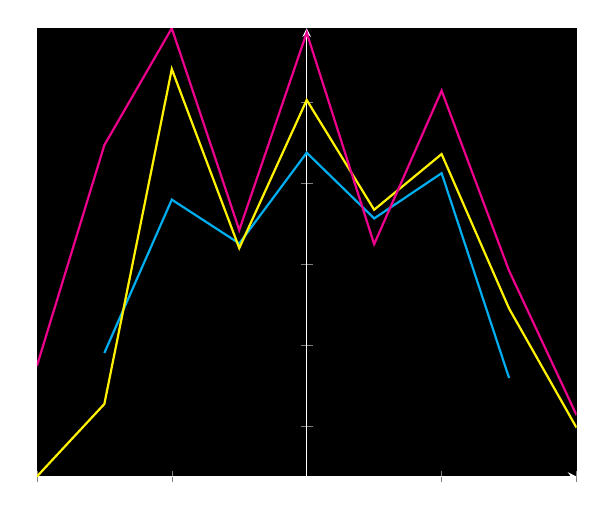
\begin{tikzpicture}[baseline]
\begin{axis}[%
axis x line = center,
axis y line = center,
xticklabels={,,},
yticklabels={,,},
scaled y ticks=false,
axis background/.style={fill=black},
axis line style={white},
]
\addplot [cyan, thick] coordinates {
(-3,	9530.667)
(-2,	19007.85)
(-1,	16297.67)
(0,	21909.00)
(1,	17846.71)
(2,	20642.69)
(3,	7984.000)
};
\addplot [yellow, thick] coordinates {
(-4,	1890.667)
(-3,	6374.111)
(-2,	27080.000)
(-1,	16011.000)
(0,	25166.666)
(1,	18383.334)
(2,	21824.000)
(3,	12277.556)
(4,	4910.222)
};
\addplot [magenta, thick] coordinates {
(-4,	8725.333)
(-3,	22378.074)
(-2,	29604.346)
(-1,	17126.518)
(0,	29328.791)
(1,	16255.111)
(2,	25744.297)
(3,	14614.123)
(4,	5688.889)
};
\end{axis}
\end{tikzpicture}
% \includegraphics[width=0.45\textwidth]{example-image}
}
\caption[USAF test chart measurement]{taorad pm. Line width: magenta: $\SI{2.19}{\micro\meter}$, yellow $\SI{1.95}{\micro\meter}$ and cyan $\SI{1.74}{\micro\meter}$. Resolution at about $\SI{1.95}{\micro\meter}$ yielding to an optical convolution of $\opticsigma = \SI{0.75}{\pixel}$.}
\label{fig:USAF}
\end{figure}
% 
\cref{fig:USAF} shows a section from a captured PM image. The highlighted areas show the key areas. A resolution of about $\SI{1.95}{\micro\meter}$ is estimated. Therefore the convolution to be applied has to be $\opticsigma = \SI{0.75}{\pixel}$ in the size of the resulting image pixel.
% 
% 
% 
\subsection{sensor gain}
%
\begin{figure}[!t]
\centering
\includegraphics[width=0.75\textwidth]{dev/gfx/2/PM_noise.png}
\caption[Noise analysis]{Noise analysis PM. $\opticgain_{\mathit{PM}} = \SI{0.1175}{}(?)$. \itodo{replot, also show microscope image}}
\label{fig:parameterModelSimGain}
\end{figure}
% 
As described in \cref{sec:ccdOptic} the optical oise has to be applied by a noise model.
In a former PhD Dissertation \cite{Wiese:887678} Hendrik Wiese measured the noise gain factor of the \ac{LAP} setup by measuring multiple times an image with a varieties of intensity values.
The same type of measurement and analysis is performed here on the \ac{PM} setup.
The results are shown in \cref{fig:parameterModelSimGain} and show a gain value of $\opticgain_{\mathit{PM}} = \SI{0.1175}{}(?)$ which is agreement to the hardware specifics \todo{check}.
% 
% 
% 
\subsection{Tissue}
% 
\begin{figure}[!t]
\captionsetup[sub]{}%position=top
\subcaptionbox{\label{fig:human:transmittance}}[0.84\textwidth]{
% \fbox{
\begin{tikzpicture}[trim axis left, trim axis right]
\begin{axis}[%
width=0.84\textwidth,
% title = {$B_1^{equ}$ in $\mu T$},
xmin=0.5,xmax=1109.5,ymin=0.5,ymax=848.5,y dir=reverse,
% point meta min=0,point meta max=6370.19,
hide axis,
colormap/blackwhite,colorbar,
]
\addplot [forget plot] graphics [xmin=0.5,xmax=1109.5,ymin=0.5,ymax=848.5] {dev/gfx/data/Vervet1818a_60mu_70ms_s0549_x00-25_y00-33_thumbnail_Transmittance-1.png};
\draw[yellow, very thick, ->] (axis cs: 500,200) -- (axis cs: 586,286);
\end{axis}
\end{tikzpicture}
\label{fig:brain_trans}
}
\\[2em]
\subcaptionbox{}[0.84\textwidth]{
\begin{tikzpicture}[trim axis left, trim axis right]
\begin{axis}[%
width=0.84\textwidth,
% title = {$B_1^{equ}$ in $\mu T$},
xmin=0.5,xmax=1109.5,ymin=0.5,ymax=848.5,y dir=reverse,
% point meta min=0,point meta max=1.0,
hide axis,
colormap/blackwhite,colorbar,
]
\addplot [forget plot] graphics [xmin=0.5,xmax=1109.5,ymin=0.5,ymax=848.5] {dev/gfx/data/Vervet1818a_60mu_70ms_s0549_x00-25_y00-33_thumbnail_Retardation-1.png};
\draw[yellow, very thick, ->] (axis cs: 500,200) -- (axis cs: 586,286);
\end{axis}
\end{tikzpicture}
\label{fig:brain_ret}
}\hspace*{\fill}
 \caption[Vervet coronal section transmittance and retardation]{Vervet coronal section. a) Transmittane, b) Retardation. The absorption coefficient and birefingence strength can be estimated from flat fibers. The corpus calusum is in a coronal section suited for this. \itodo{histograms?}}
\label{fig:brain_ret_trans}
\end{figure}
% 
\begin{figure}[!t]
\centering
\subcaptionbox{transmittance}[.95\textwidth]{
\includegraphics[width=0.95\textwidth]{dev/gfx/2/transmittance_PM_Vervet.pdf}} %\hfill
\subcaptionbox{retardation}[.95\textwidth]{
\includegraphics[width=0.95\textwidth]{dev/gfx/2/retardation_PM_Vervet.pdf}}
\caption{simulations for Vervet PM tissue for different absorption coef and birefringence values.}
\label{fig:parameterModelSim}
\end{figure}
% 
% 
% 
\subsection{voxel size \texorpdfstring{\voxels{}}{}}
% 
% % 
In \cref{sec:dv_generator} the \voxelsize{} parameter $\voxels$ was introduced.
% This parameter has a major role in the accuracy of the results.
% It does not only account for the discretization accuracy of the 3d model, but also for the number of light rays.
% The impact is visualie shown in \cref{fig:vectorfield_disc_error}.
% It is cleare that 
% 
% TODO: anhang?
% \begin{figure}[p]
% \centering
% \includegraphics[width=\textwidth, page=4]{dev/gfx/2/voxel_size_plots_data_0.pdf}
% \caption[voxel size model without noise]{without noise \dummy{}}
% \label{fig:voxelsize}
% \end{figure}
% 
\begin{figure}[p]
\centering
\includegraphics[width=\textwidth, page=4]{dev/gfx/2/voxel_size_plots_data_1.pdf}
\caption[voxel size model with noise]{with noise \dummy{}}
\label{fig:voxelsizeNoise}
\end{figure}
